\documentclass{report}

\usepackage[utf8]{inputenc} % Charakter-Kodierung
\usepackage[german]{babel} % Sprache

\usepackage[table,xcdraw]{xcolor} % Tabellen Farben
\usepackage{tabularx} % Dynamische Tabellenbreite
\usepackage{tcolorbox} % Graue Boxen
\usepackage{hyperref} % url Umgebung
\usepackage{todonotes} % Notizen
\usepackage{natbib} % Bibliographie
\usepackage{fancyhdr} % Header und Footer
\usepackage{multirow} % Multizeile
\usepackage{geometry} % Page layout
\usepackage{color} % Text Farben

% Page layout
\geometry{
	bottom=3.5cm,
	headheight=180pt
}

% Nummerierung der ersten Seiten verhindern
\pagenumbering{gobble}

% Bibstyle
\bibliographystyle{plain}

% Header / Footer
\fancypagestyle{plain}{
	\fancyhf{}% Clear header/footer
	\fancyhead[R]{
\includegraphics[width=4cm]{img/cau-logo-2017}} % Rechter header
	\fancyhead[L]{\leftmark} % Linker header
	\fancyfoot[R]{\thepage} % Rechter footer
	\fancyfoot[L]{
\includegraphics[width=1cm]{img/se-logo}} % Linker footer	
}
\pagestyle{plain}

\renewcommand{\headrulewidth}{0.5pt} % Unnötige Informationen der Kapitelangabe
\renewcommand{\footrulewidth}{0.2pt} % entfernen
\renewcommand{\chaptermark}[1]{\markboth{{#1}}{}}




% Zahlen für Fußnoten
\renewcommand{\thefootnote}{\arabic{footnote}}
\renewcommand{\thempfootnote}{\arabic{mpfootnote}}

%%%%% Ausfüllen %%%%%

\newcommand{\gruppenname}{Gruppe WSP3 1}
\newcommand{\projektname}{Projekt GoGross}
\newcommand{\semester}{Wintersemester 2023/24}



% Titelseite

\title{
	\vspace*{-3cm}
	Entwurfsdokumentation\\
	\projektname\\
	-\\
	\color{gray}
	Softwareprojekt \semester\\
	\gruppenname\\
	\vspace*{5mm}
	
\includegraphics[width=\textwidth]{img/logo}
}

\author{
	\begin{tabular}{r l@{\hspace{8\tabcolsep}} r} 
		Lia & Lenckowski & \multirow{8}{*}{ 
\includegraphics{img/se-logo} } \\
		Leon & Klausing \\
		Matheus & Kolzarek \\
		Noe & Baumann \\
		Shutong & Sun \\
		Til & Schmidt \\
		Tjark-Morten & Thies \\
		Yuri & Hassink \\
	\end{tabular}
}

\date{\today}

% Dokument

\begin{document}
	\maketitle
	\tableofcontents 

	\chapter{Einleitung}\label{chp:einleitung}
	\pagenumbering{arabic} % Nummerierung starten
	\thispagestyle{fancy}
	\section{Entwicklungsumgebung}\label{sec:entwicklungsumgebung}


\begin{table}[h]
	\centering
	\begin{tabularx}{\textwidth}{l l X}
		\rowcolor[HTML]{C0C0C0} 
		\textbf{Software} & \textbf{Version} & \textbf{URL} \\
		Python & 3.11.X & \url{https://www.python.org/} \\
		\rowcolor[HTML]{E7E7E7} 
		Docker & 25.0.3 & \url{https://www.docker.com/} \\
		Git & 2.44.0 & \url{https://git-scm.com/} \\
		\rowcolor[HTML]{E7E7E7} 
		VSCode & 1.84.0& \url{https://code.visualstudio.com/} \\
		Flask & 3.0.2 & \url{https://flask.palletsprojects.com/en/3.0.x/} \\
		\rowcolor[HTML]{E7E7E7} 
		SQLite & 3.45.1 & \url{https://www.sqlite.org/} \\
		nginx & 1.21.3 & \url{https://www.nginx.com/} \\
		\rowcolor[HTML]{E7E7E7} 
		uWSGI & 2.0.24 & \url{https://uwsgi-docs.readthedocs.io/en/latest/} \\
		Open JDK & 11.0.22 & \url{https://www.oracle.com/java/technologies/downloads} \\
		\rowcolor[HTML]{E7E7E7} 
		Android Studio & 2023.2.1 & \url{https://developer.android.com/studio} \\
	\end{tabularx}
	\caption{Enwicklungsumgebung}
	\label{table:entwicklungsumgebung}
\end{table}


	\chapter{Team-Aufteilung}
	\thispagestyle{fancy}
	\begin{tabular}{ll}
 \rowcolor[HTML]{E7E7E7}
 \textbf{Name} & \textbf{Zuständigkeit} \\ \hline
 Lia & 1. CI/CD Tests, 2. Backend \\
 \rowcolor[HTML]{E7E7E7}
 Leon & 1. Frontend, 2. Testen \\
 Matheus & Backend \\
 \rowcolor[HTML]{E7E7E7}
 Noe & 1. Frontend APP, 2. Backend \\
 Shutong & 1. Frontend, 2. Backend \\
 \rowcolor[HTML]{E7E7E7}
 Til & 1. Frontend 2. Backend \\
 Tjark-Morten & 1. Frontend 2. Backend \\
 \rowcolor[HTML]{E7E7E7}
 Yuri & Backend \\
\end{tabular}

\bigskip


	\chapter{Komponentendiagramme}\label{chp:komponentendiagramme}
	\thispagestyle{fancy}
	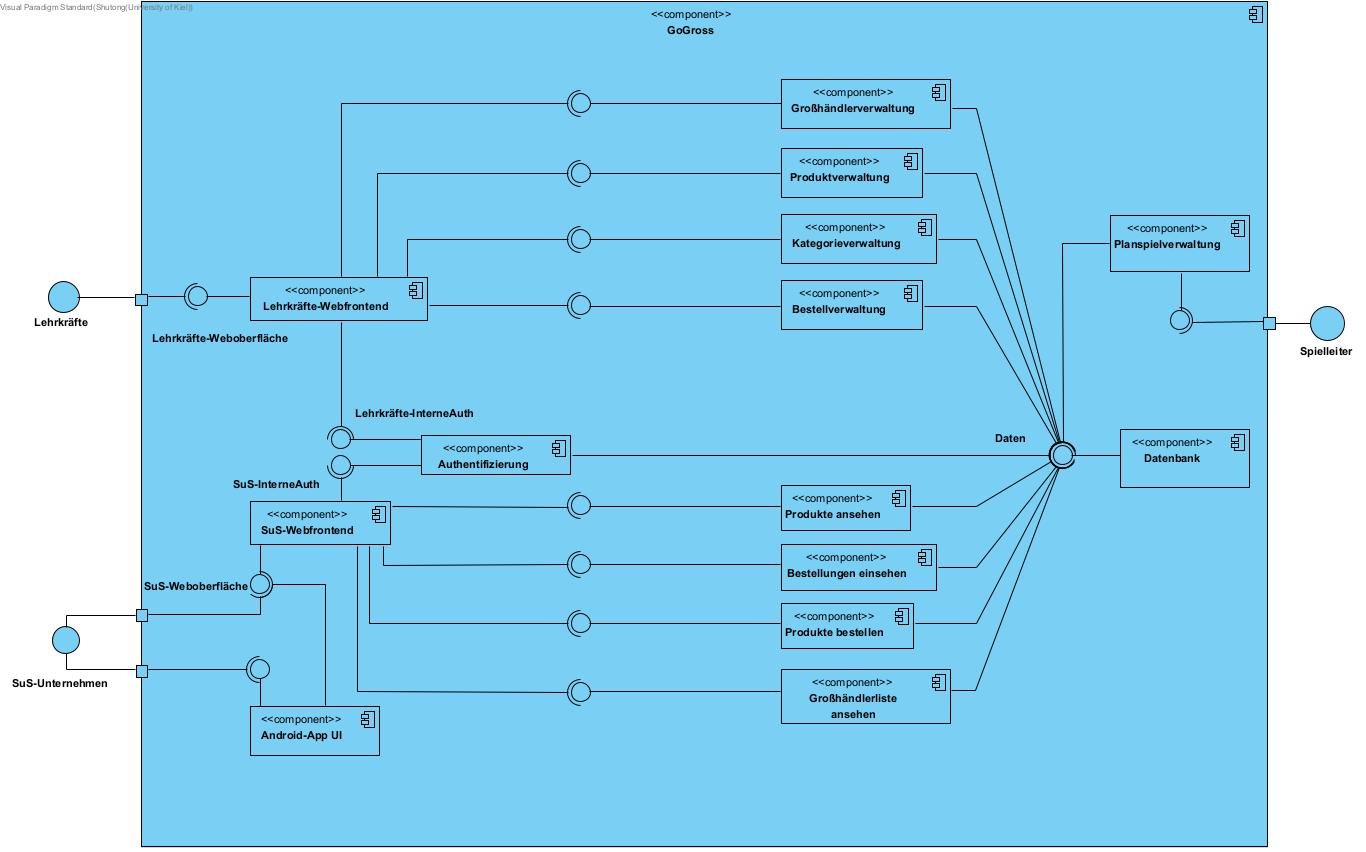
\includegraphics[width=\textwidth]{img/Component}
\label{fig: GoGross Komponentendiagramm}

\begin{itemize}
    \item Der Spielleiter kann alle Planspiele über die Kommandozeile verwalten. Die Verwaltung umfasst die Erstellung, das Beenden sowie den Import und Export von Spielständen.
    \item Die Lehrkräfte nutzen eine über HTTPS gesicherte Weboberfläche, die über eine Authentifizierungskomponente gesichert ist. Nach erfolgreicher Authentifizierung können diese auf verschiedene Verwaltungskomponenten zugreifen. Diese ermöglichen das Management von Großhändlern, Produkten, Kategorien und Bestellungen. Wie zum Beispiel das Löschen, Hinzufügen, Importieren oder Exportieren.
\newpage
    \item SuS-Unternehmen verwenden entweder eine Weboberfläche oder eine auf der Weboberfläche basierende Android-Anwendung, um sich zu authentifizieren und anschließend Zugriff auf verschiedene Bestellkomponenten zu erhalten. So können diese Großhändler, Produkte und Bestellungen ansehen sowie Bestellungen tätigen. 
    \item Die Authentifizierungskomponente gewährleistet einen sicheren Zugang für Lehrkräfte und SuS-Unternehmen. Diese reguliert den Zugriff mithilfe der gespeicherten Benutzerdaten in der Datenbank und sichert somit die Integrität sowie Sicherheit des Systems.
    \item Das GoGross System wird von einer internen Datenbankkomponente gestützt, welche relevante Informationen und Beziehungen speichert. Diese Datenbank wird von den verschiedenen Komponenten zur Ausführung ihrer spezifischen Aufgaben abgefragt und verändert. 
\end{itemize}

	\chapter{Verteilungsdiagramm}\label{chp:verteilungsdiagramm}
	\thispagestyle{fancy}
	\begin{itemize}
	\item Alle Komponenten des Systems werden auf dem Webserver des RBZ gehostet.
	\item Um unsere Web-Anwendung zu nutzen, muss Docker auf dem Webserver laufen.
	\item Alle Daten werden mittels SQLite auf dem Webserver gespeichert.
	\item Alle HTTPS-Anfragen werden mittels nginx auf den Webserver geleitet.
\end{itemize}


\begin{figure}[h]
	\centering
	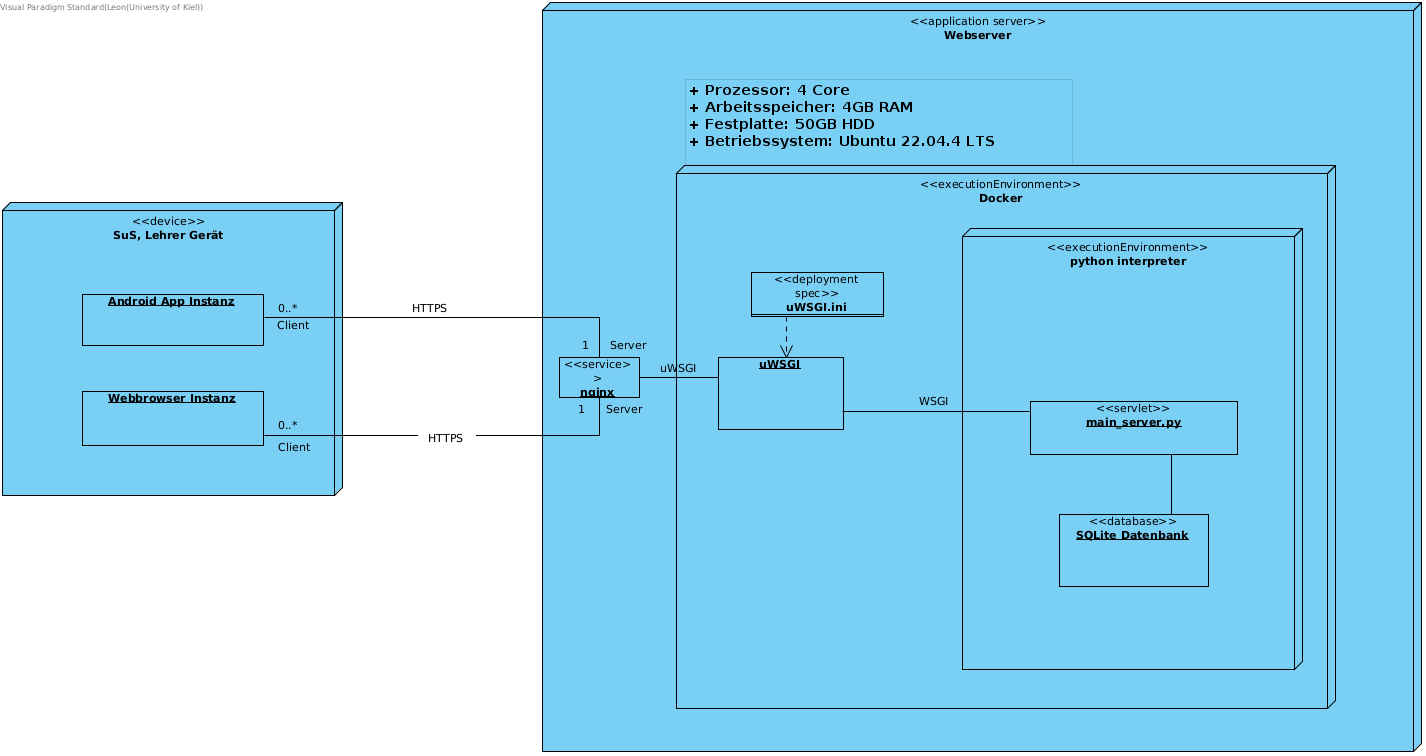
\includegraphics[width=\textwidth]{img/Verteilungsdiagramm.png}

	\caption{Verteilungsdiagramm}
	\label{fig:verteilungsdiagramm}
\end{figure}



	\chapter{Klassendiagramme oder API-Beschreibung}\label{chp:klassendiagramme-api}
	\thispagestyle{fancy}
	Auf die Diagramme folgt jeweils eine textuelle Beschreibung aller Endpunkte. \\
Darin stellen Pfadteile in angle brackets (\texttt{<x>}) nötige, und Pfadteile in square brackets (\texttt{[x]}) optionale Parameter dar.\\

\section{API-Diagramme für Lehrer}
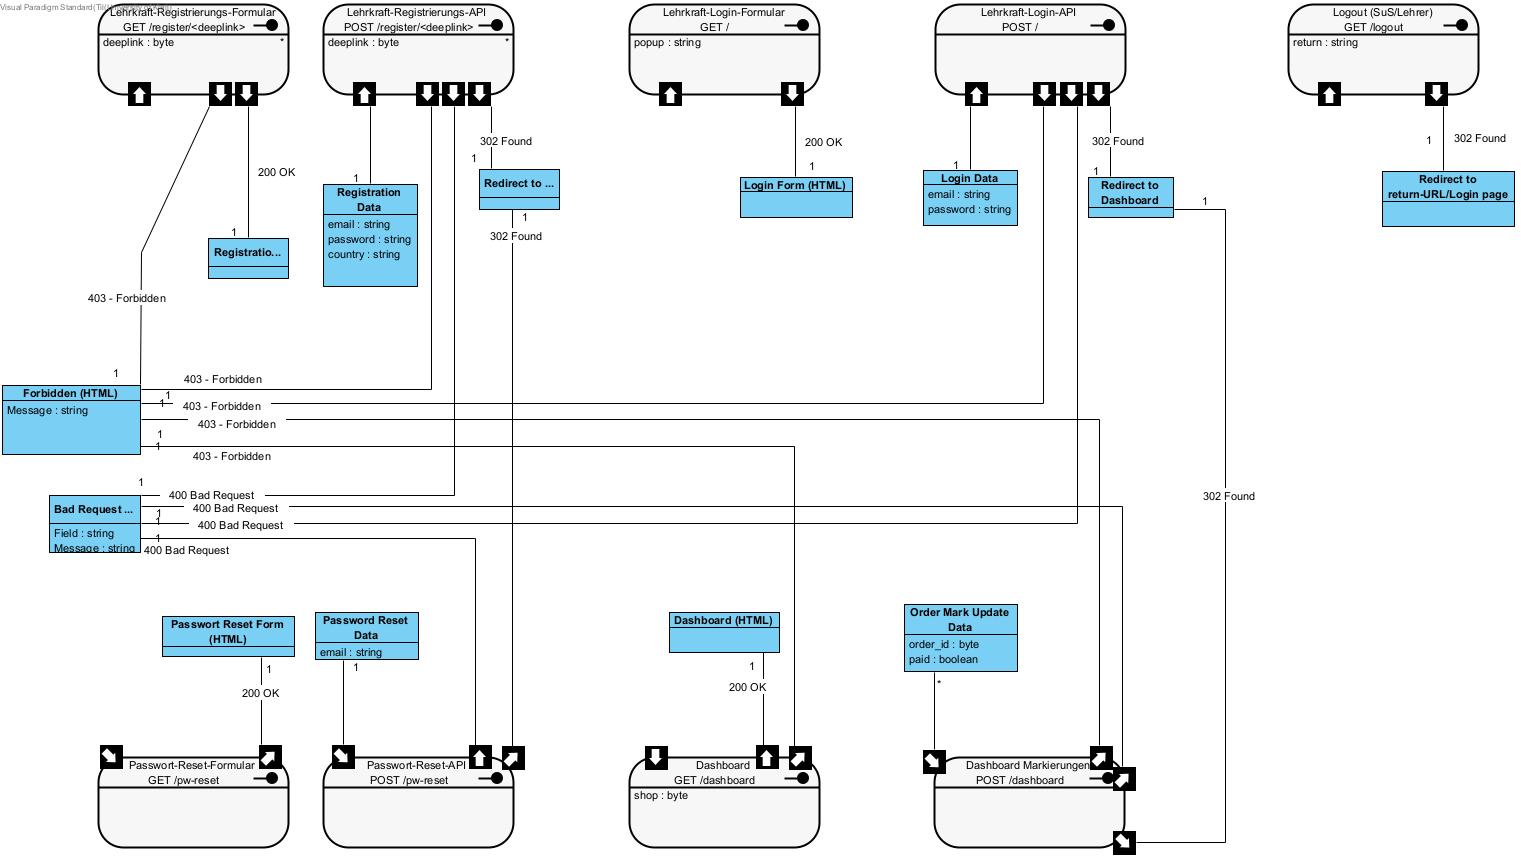
\includegraphics[width=\textwidth]{img/api-lehrkraft-login}
\begin{itemize}
	\item \texttt{/register/<deeplink>}: Die Lehrer-Registrierung ist nur über deinen Deeplink erreichbar.
		\begin{itemize}
			\item GET: Registrierungsformular.
			\item POST: Hier wird ein JSON-Body mit den Daten aus dem Registrierungsformular erwartet. Erfolg führt zu einer Weiterleitung zu \texttt{/?popup=Registrierung+Erfolgreich}.
		\end{itemize}
	\item \texttt{/?[popup=<TEXT>]}: Lehrkraft-Login.
		\begin{itemize}
			\item GET: Login-Formular. Falls ein popup-Text gegeben wird, wird dieser angezeigt.
			\item POST: Hier wird ein JSON-Body mit Login-Daten erwartet. Erfolg führt zu einer Weiterleitung zu \texttt{/dashboard}.
		\end{itemize}
	\item \texttt{/pw-reset}: Lehrkraft-Passwort-Reset.
		\begin{itemize}
			\item GET: Passwort-Reset-Formular.
			\item POST: Hier wird ein JSON-Body mit der E-Mail, dessen zugehöriger Account sein Passwort zurückgesetzt haben soll, erwartet. Erfolg führt zu einer Weiterleitung zu \texttt{/}.
		\end{itemize}
	\item \texttt{/logout?[return=<URL>]}: Logout.
		\begin{itemize}
			\item GET: Aufruf führt zum Logout, sowohl von Lehrkraft- als auch SuS-Sessions. Falls angegeben, wird danach zur return-URL weitergeleitet, sonst zu \texttt{/}.
		\end{itemize}
	\item \texttt{/dashboard?[shop=<ID>]}: Lehrkraft-Dashboard. Nur nach Login mit Lehreraccount erreichbar. Angabe des shop-parameters filtert die angezeigte Bestellungsliste auf Bestellungen bei dem gegebenen Shop.
		\begin{itemize}
			\item GET: Lehrkraft-Dashboard. Es werden nur Daten zu den Großhändlern aus dem Land des Lehrkraftaccounts dargestellt.
			\item POST: Hier wird ein JSON-Body erwartet, der für eine Untermenge an Bestellungen angibt, ob sie als bezahlt oder unbezahlt zu markieren sind. Erfolg führt zu einer Weiterleitung zu \texttt{/dashboard}.
		\end{itemize}
\end{itemize}

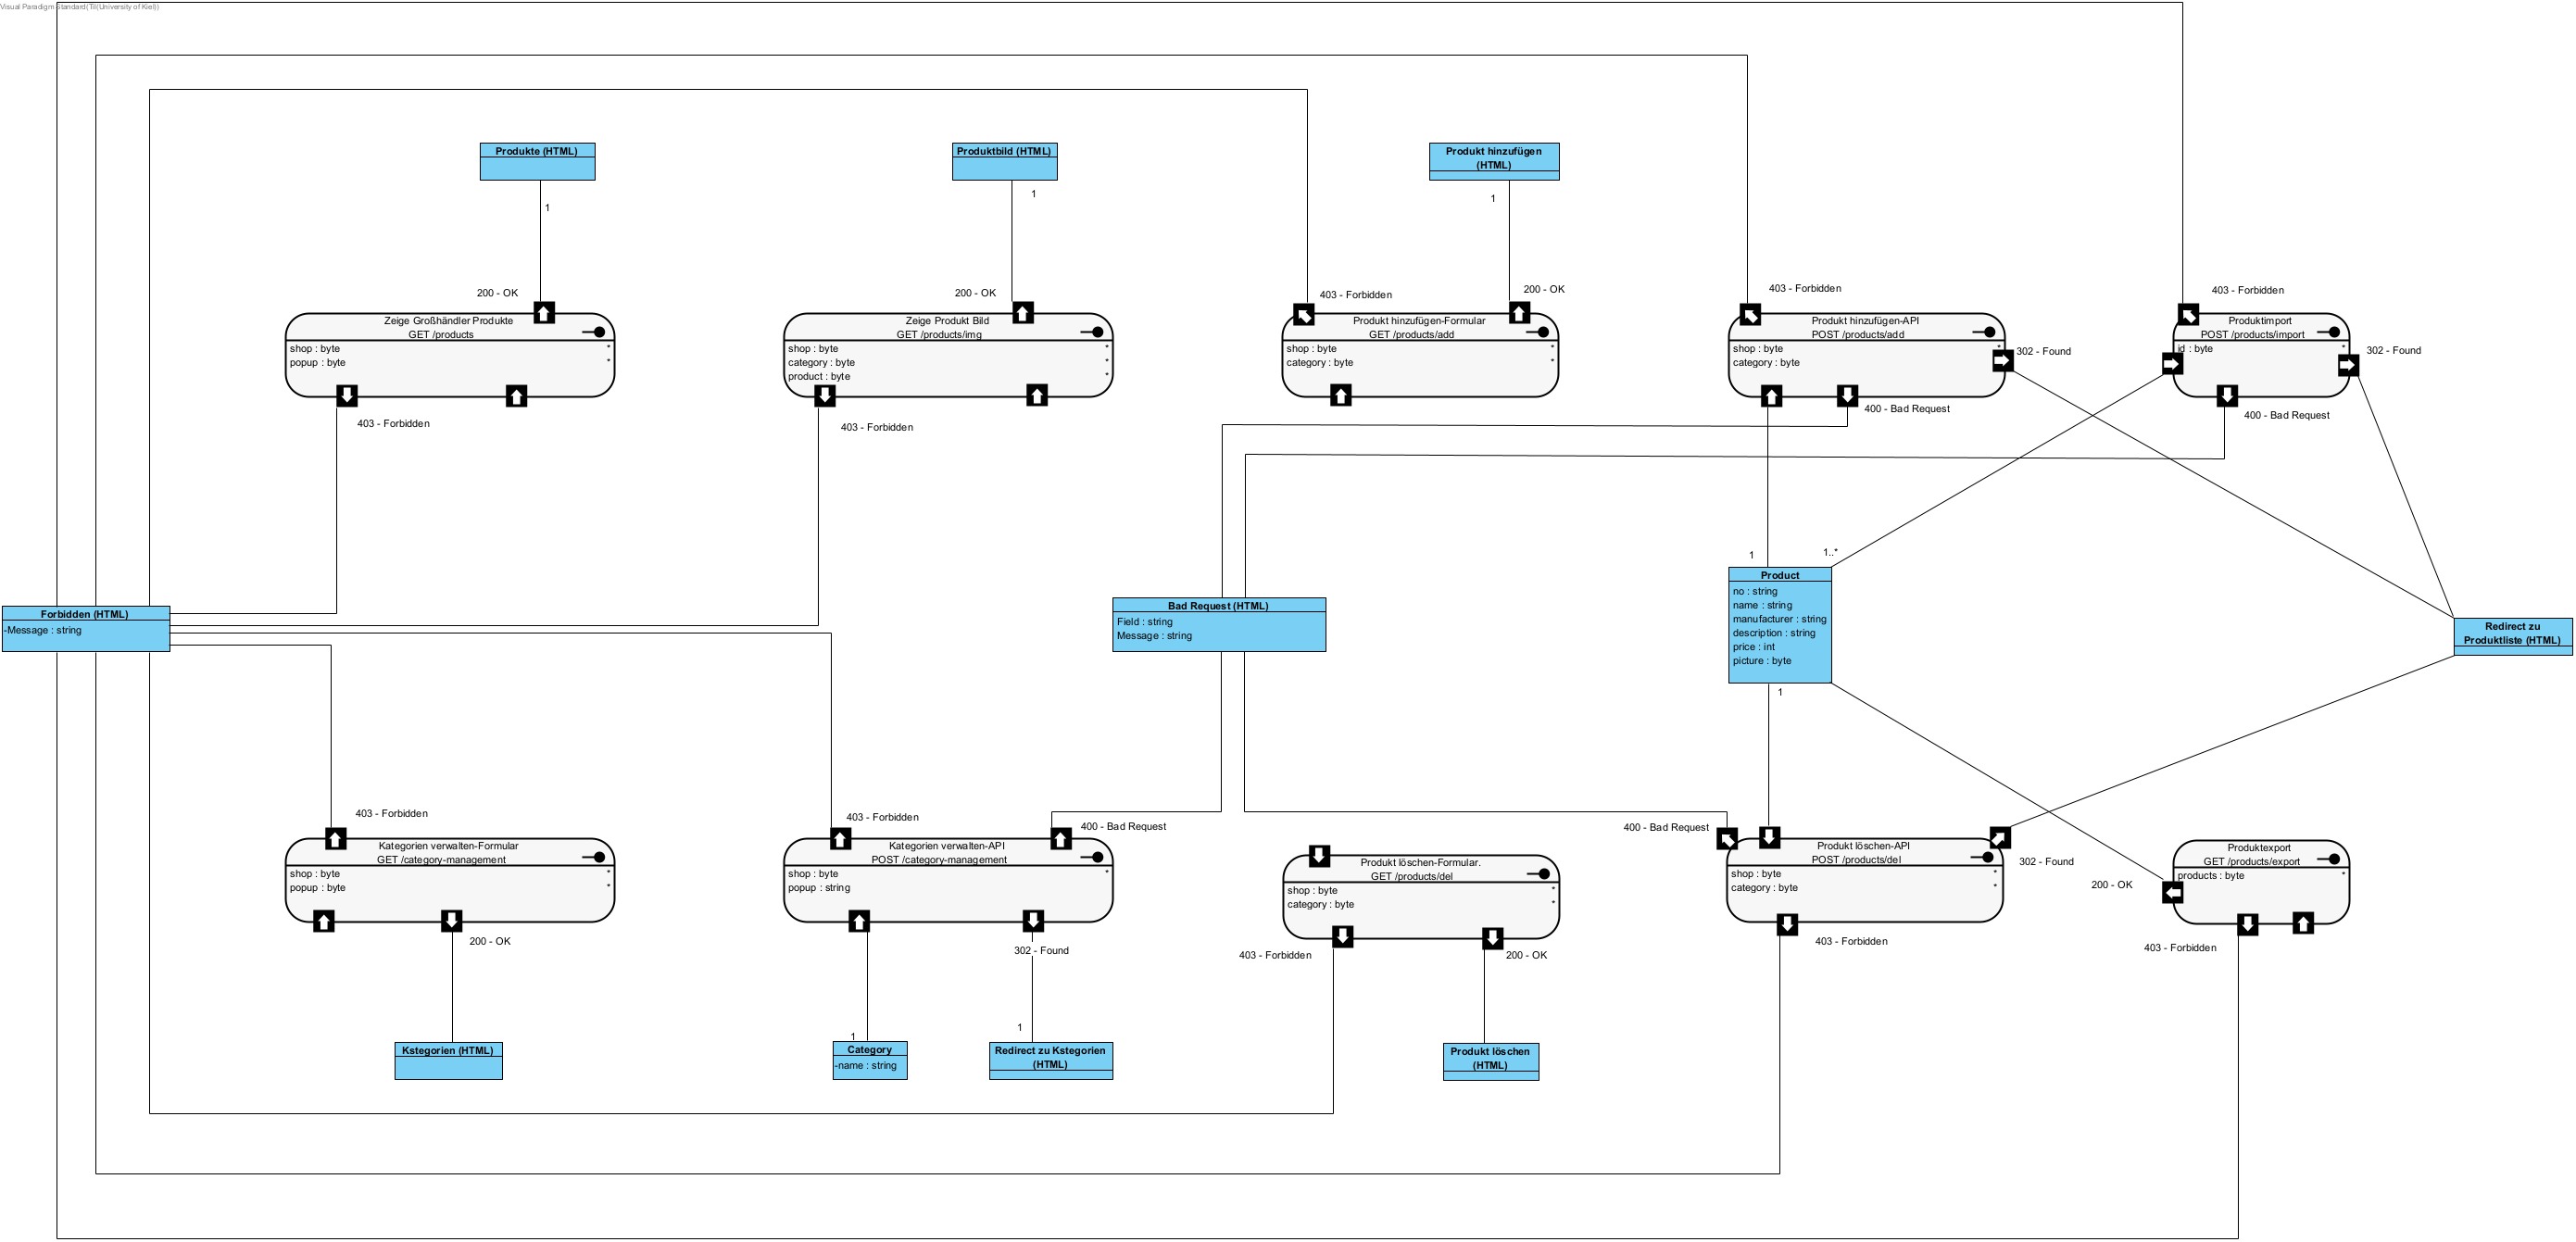
\includegraphics[width=\textwidth]{img/api-lehrkraft-produkt-kategorie}
Die folgenden Endpoints sind je nur mit einem Lehreraccount erreichbar, dessen Land zu evtl. angegebenen Großhändlern/Produkten passt.
\begin{itemize}
	\item \texttt{/products?shop=<ID>[\&category=<ID>\&popup=<ID>]}: Produktlisten aus Lehrkraft-Sicht.
		\begin{itemize}
			\item GET: Zeigt die Produktliste des angegeben Shops an. Je nach Parametern sind Produkte nach einer Kategorie gefiltert und/oder es wird ein Popup mit Text angezeigt.
		\end{itemize}
	\item \texttt{/products/img?product=<ID>}: Produktbilder.
		\begin{itemize}
			\item GET: Gibt als je natives Format das Bild des angegebenen Produktes zurück.
		\end{itemize}
	\item \texttt{/products/export?products=<ID>[,ID2[,ID3[...]]]}: Produktexport.
		\begin{itemize}
			\item GET: Gibt als JSON-Liste die angegebenen Produkte zurück.
		\end{itemize}
	\item \texttt{/products/import?shop=<ID>}: Produktimport.
		\begin{itemize}
			\item POST: Erwartet eine JSON-Liste an Produkten, die zu dem angegebenen Großhändler hinzugefügt werden.
		\end{itemize}
	\item \texttt{/products/add?shop=<ID>}: Produkt-Hinzufügungs-UI.
		\begin{itemize}
			\item GET: UI zum hinzufügen von einem Produkt.
			\item POST: Erwartet JSON mit Produktdaten \& Bild, und fügt es beim angegebenen shop in einer im JSON angegebenen Kategorie hinzu.
		\end{itemize}
	\item \texttt{/products/del?shop=<ID>}: Produktlöschungs-API.
		\begin{itemize}
			\item POST: Erwartet JSON mit Produkt-ID. Bei erfolg wird zu\\
				\texttt{/products?shop=ID\&popup=Erfolgreich+Gelöscht} weitergeleitet.
		\end{itemize}
	\item \texttt{/category-management?shop=<ID>[\&popup=<TEXT>]}: UI fürs hinzufügen/löschen von Kategorien.
		\begin{itemize}
			\item GET: UI zum Hinzufügen/Löschen von Kategorien, wobei man Änderungen erst speichern muss (was zu einem POST an dieselbe URL führt). Ein gegebenes Popup wird gezeigt.
			\item POST: Erwartet als JSON eine Liste an hinzugefügten \& gelöschten Kategorien. Bei Erfolg wird auf \texttt{/category-management?shop=ID\&popup=Erfolgreich+Geändert} weitergeleitet.
		\end{itemize}
\end{itemize}

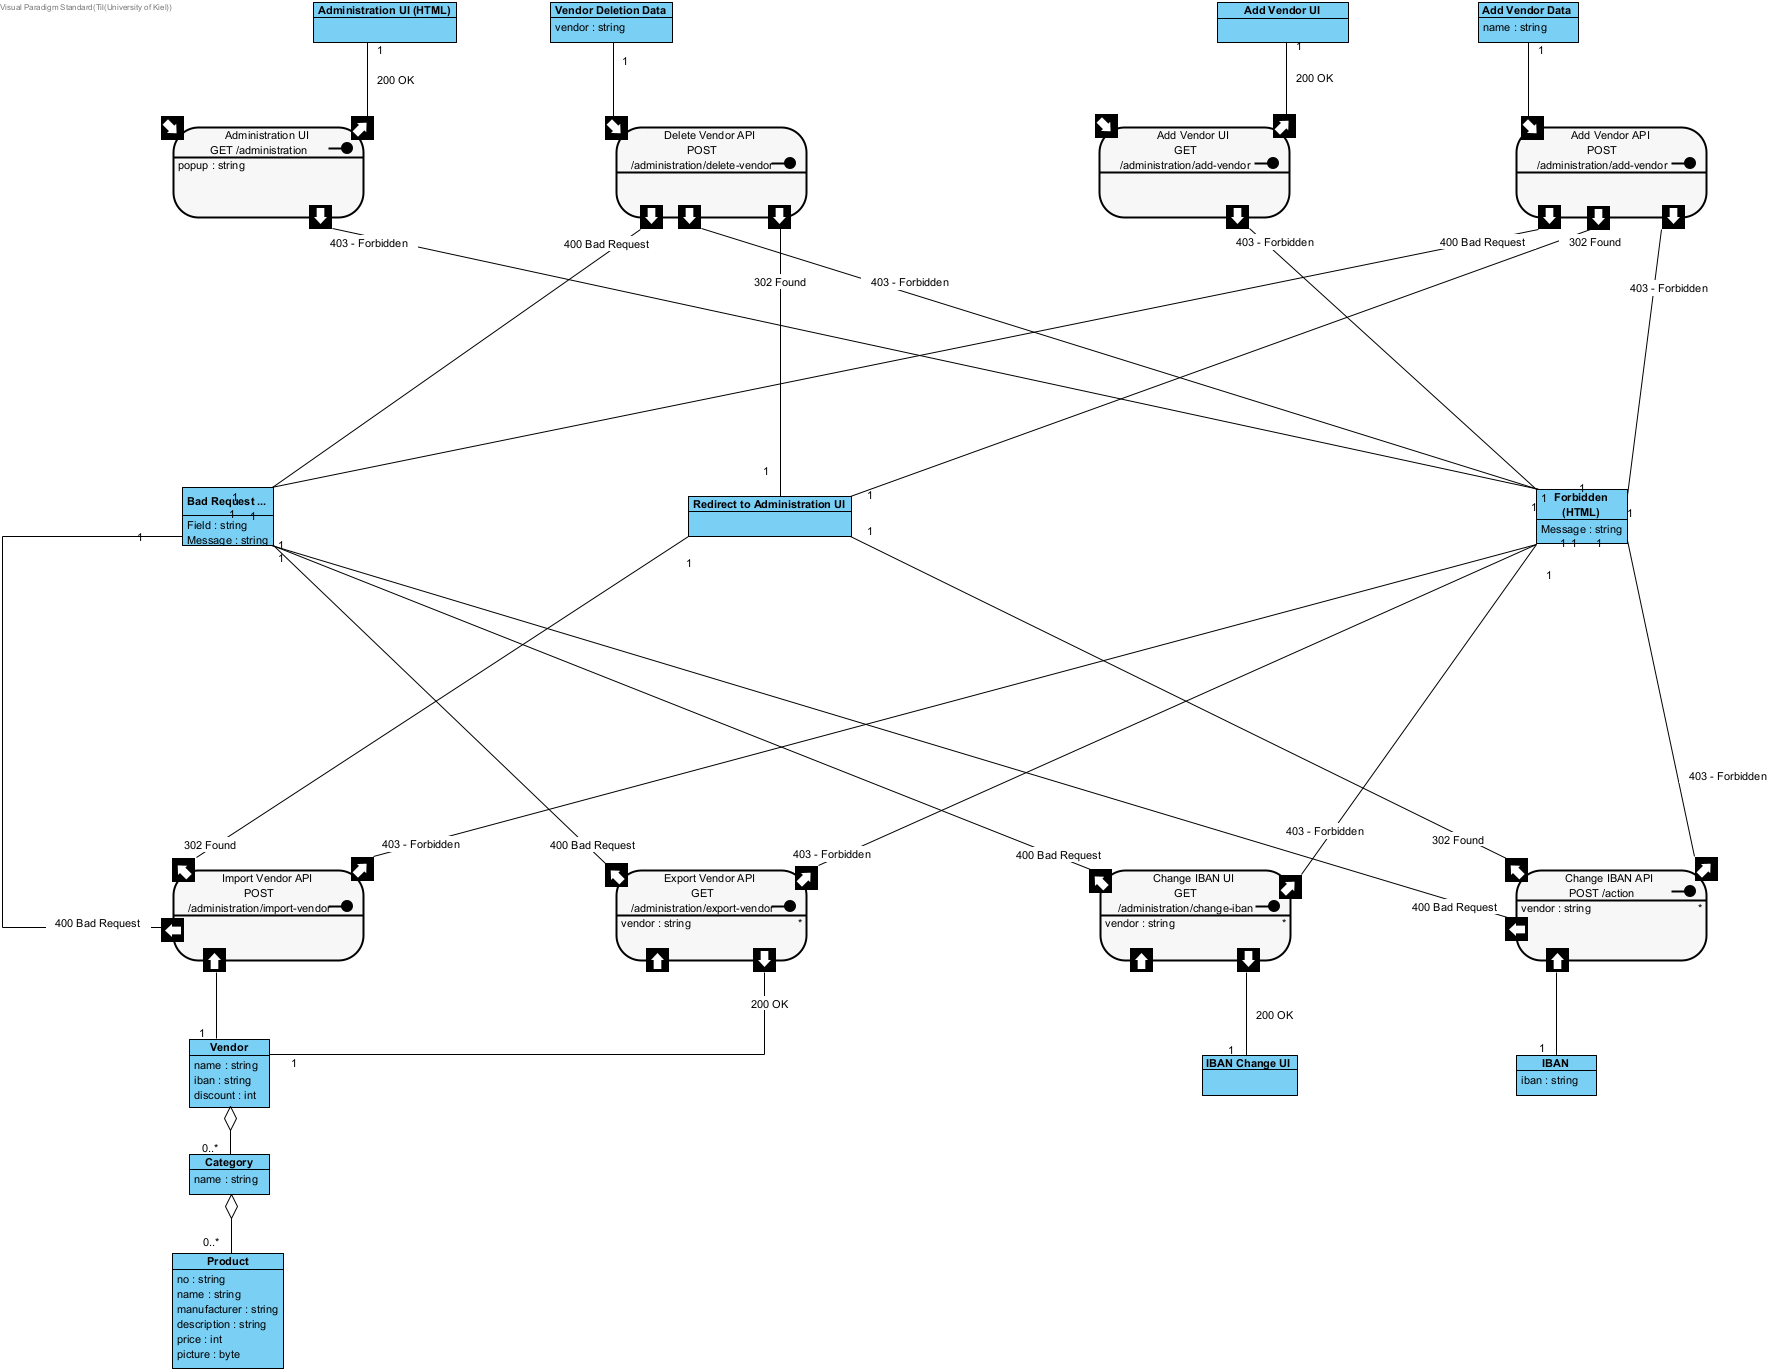
\includegraphics[width=\textwidth]{img/api-lehrkraft-administration}
\begin{itemize}
	\item \texttt{/administration?[popup=<TEXT>]}: UI zum verwalten von Großhändlern.
		\begin{itemize}
			\item GET: UI zum Hinzufügen/Löschen/Bearbeiten/Import/Export von Großhändlern. Ein gegebenes Popup wird gezeigt.
		\end{itemize}
	\item \texttt{/administration/add-vendor}: UI zum hinzufügen von vendors.
		\begin{itemize}
			\item GET: UI zum hinzufügen von Großhändlern.
			\item POST: Erwartet JSON mit Großhändler-Name, -Bild und -IBAN. Bei Erfolg wird auf \texttt{/administration?popup=Erfolgreich+Hinzugefügt} weitergeleitet.
		\end{itemize}
	\item \texttt{/administration/delete-vendor}: Großhändler-Löschungs-API.
		\begin{itemize}
			\item POST: Erwartet JSON mit Großhändler-ID, und löscht ihn \& zugehörige Produkte, Kategorien, Bestellungen \& Rechnungen. Bei Erfolg wird auf \texttt{/administration?popup=Erfolgreich+Gelöscht} weitergeleitet.
		\end{itemize}
	\item \texttt{/administration/export-vendor?shop=<ID>}: Großhändler-Export-API.
		\begin{itemize}
			\item GET: Gibt einen vendor mit allen Kategorien und Produkten, aber ohne zugehörigen Accounts und Bestellungen als JSON zurück.
		\end{itemize}
	\item \texttt{/administration/import-vendor}: Großhändler-Import-API.
		\begin{itemize}
			\item POST: Erwartet eine Datei, die durch einen Großhändler-Export erstellt wurde. Bei Erfolg wird auf \texttt{/administration?popup=Erfolgreich+Importiert} weitergeleitet.
		\end{itemize}
	\item \texttt{/administration/change-iban?shop=<ID>}: Großhändler-Bearbeitungs-UI.
		\begin{itemize}
			\item GET: Großhändler-Bearbeitungs-UI. Dabei sind auf jeden fall IBAN, später vielleicht auch das Logo einstellbar.
			\item POST: Erwartet JSON mit einer neuen IBAN und/oder einem neuen Logo. Bei Erfolg wird auf \texttt{/administration?popup=Erfolgreich+Geändert} weitergeleitet.
		\end{itemize}
\end{itemize}


\section{API-Diagramme für SuS}
Hier verzichten wir aufs Darstellen von Registrierung/Login, da es im wesentlichen gleich wie bei Lehrkräften aufgebaut ist, außer das alle pfade einen deeplink als Präfix haben.

\begin{itemize}
	\item \texttt{/<deeplink>}: Großhändlerübersicht-UI
		\begin{itemize}
			\item GET: UI, welche die Übersicht aller Großhändler des zugehörigen deeplinks anzeigt.
		\end{itemize}
	\item \texttt{/<deeplink>/invoice?id=<ID>}: Invoice-PDF
		\begin{itemize}
			\item GET: Zeigt Invoice als PDF an.
		\end{itemize}
	\item \texttt{/<deeplink>/catalog?[category=<ID>][\&popup=<TEXT>]}: Produktübersicht-UI
		\begin{itemize}
			\item GET: UI zur Übersicht der Produkte eines Großhändlers. Ein gegebenes Popup wird gezeigt.
		\end{itemize}
	\item \texttt{/<deeplink>/img?product=<ID>}: Produktbilder.
		\begin{itemize}
			\item GET: Gibt als je natives Format das Bild des angegebenen Produktes zurück.
		\end{itemize}
	\item \texttt{/<deeplink>/add-to-cart?[return-cat=<ID>]}: UI zum Hinzufügen von Produkten aus dem Warenkorb
		\begin{itemize}
			\item POST: Erwartet JSON mit Produkt-ID und Anzahl. Bei Erfolg wird auf \texttt{/<deeplink>/catalog?[category=<ID>]popup=Erfolgreich+Hinzugefügt} weitergeleitet.
		\end{itemize}
	\item \texttt{/<deeplink>/cat?[popup=<TEXT>]}: Warenkorb-UI
		\begin{itemize}
			\item GET: UI zur Ansicht des Warenkorbs. Ein gegebenes Popup wird gezeigt.
		\end{itemize}
	\item \texttt{/<deeplink>/del-from-cart}: UI zum Löschen von Produkten aus dem Warenkorb
		\begin{itemize}
			\item POST: Erwartet JSON mit Produkt-ID und löscht das Produkt. Bei Erfolg wird auf \texttt{/<deeplink>/car?popup=Erfolgreich+Gelöscht} weitergeleitet.
		\end{itemize}
	\item \texttt{/<deeplink>/checkout}: Bestellen-UI
		\begin{itemize}
			\item POST: Erwartet ein leeres JSON. Bei Erfolg wird auf die erstellte Invoice weitergeleitet.
		\end{itemize}
\end{itemize}

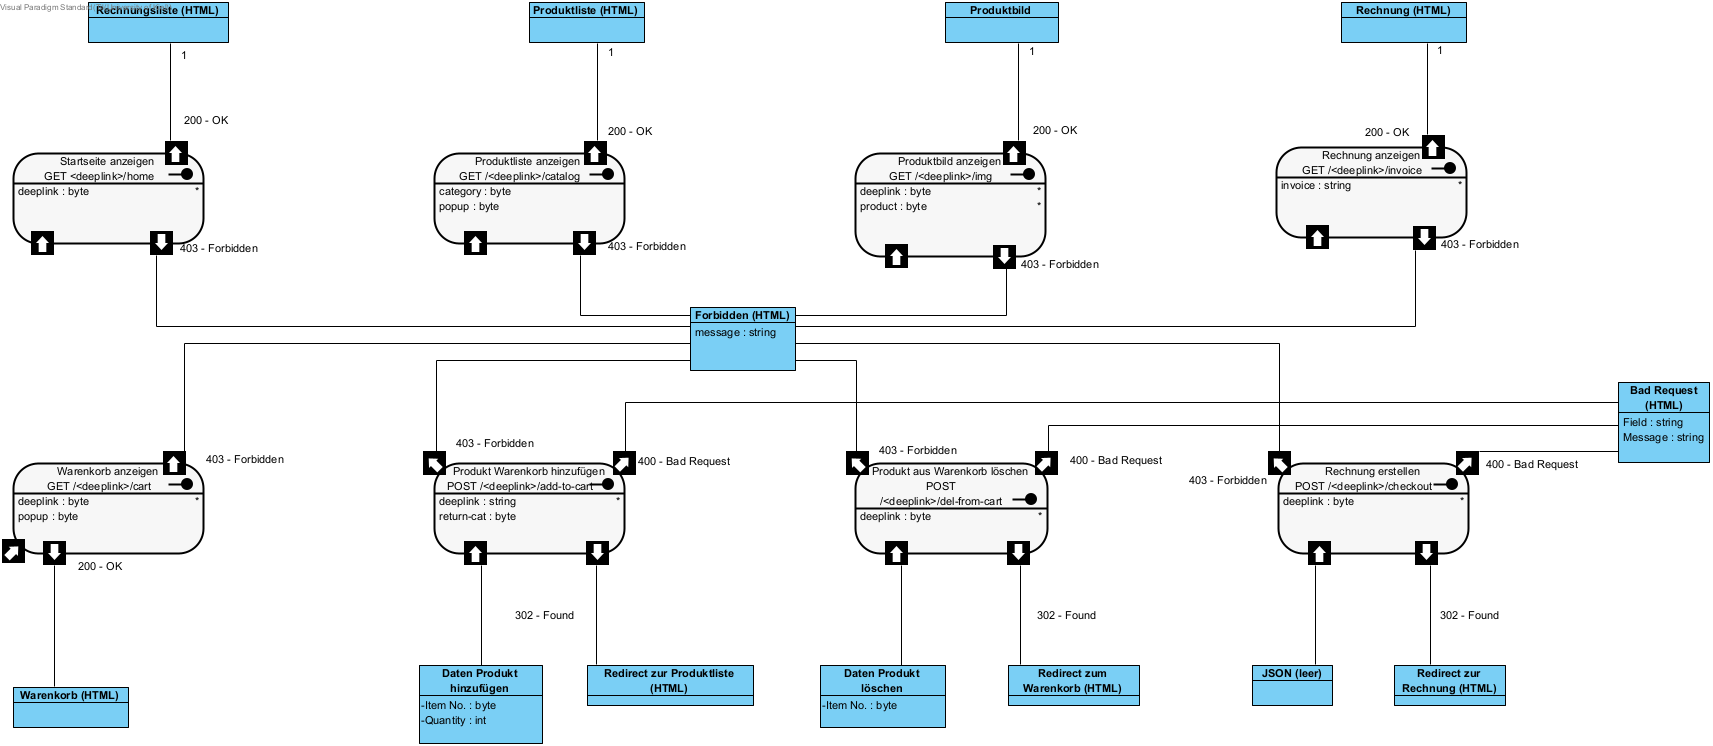
\includegraphics[width=\textwidth]{img/api-sus}


	\chapter{Sequenzdiagramme}\label{chp:sequenzdiagramme}
	\thispagestyle{fancy}
	Es ist wichtig bei allen folgenden Sequenzdiagrammen zu beachten, dass die sonst als lifelines bekannten Objekte hier als "usageline" interpretiert werden sollten.

\section{SuS-Login}
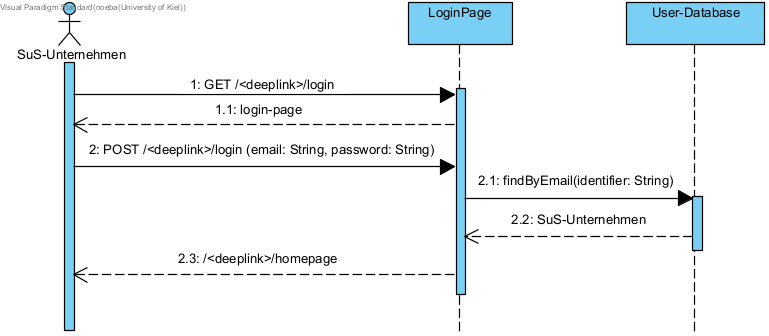
\includegraphics[width=\textwidth]{img/sequence-sus-login}
\label{fig: SuS-Login Sequenzdiagramm}
Um sich als SuS-Unternehmen einzuloggen wird vom oder von der Nutzer*in erst die LoginPage via Deeplink abgefragt. An diese werden danach die Logindaten gesendet, welche diese weiter an die Datenbank leitet um den oder die Nutzer*in zu authentifizieren. Ist die Authentifikation erfolgreich, so gibt die Datenbank den SuS-Unternehmen-Account zurück an die LoginPage und diese leitet den oder die Nutzer*in weiter zu der Shop-Homepage.

\section{SuS Produkt kaufen}
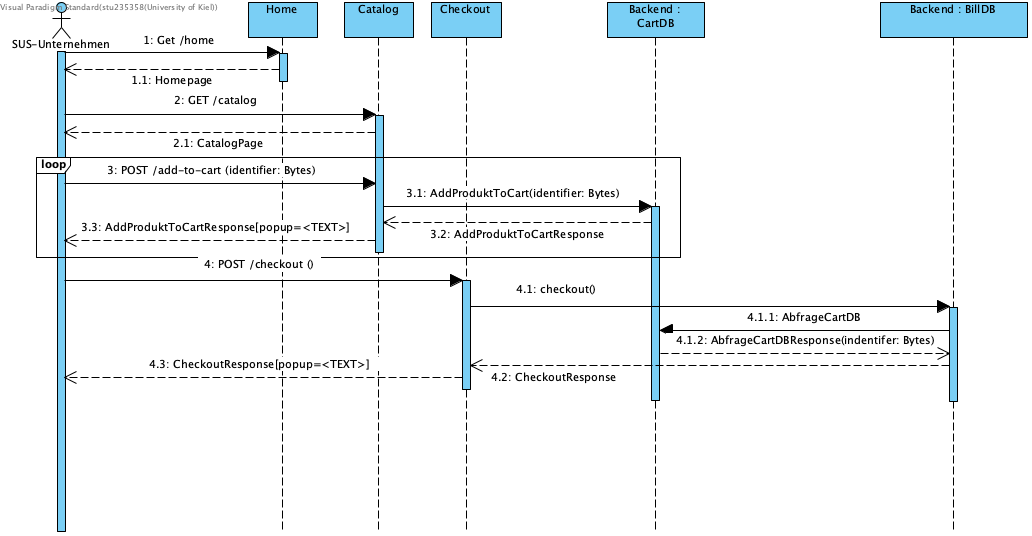
\includegraphics[width=\textwidth]{img/sequence-sus-buy-product}
\label{fig: SuS Produkt kaufen Sequenzdiagramm}
Dieses Sequenzdiagramm beschreibt den Prozess vom Produkt anschauen bis hin zum Kauf. Nachdem der oder die Nutzer*in die Homepage abgefragt und erhalten hat, fragt diese*r die Katalogsseite ab. Hier kann nun ein Produkt in Warenkorb hinzugefügt werden. Produkt \& session werden an eine Backend-Komponente weitergeleitet, welche den aktuellen Warenkorb für jeden Nutzer speichert. Werden mehr als nur eine Instanz des Produkts gleichzeitig dem Warenkorb hinzugefügt, so wird dieser loop entsprechend oft durchgeführt. Entscheidet sich der oder die Nutzer*in den Warenkorb zu bestellen, so schickt er/sie über die Weboberfläche einen Anfrage an einen Checkout-Endpoint, welcher diese and die Bill-Datenbank im Backend sendet. Die Bill-Datenbank fragt dann bei der Cart-Datenbank an, welche Objekte sich im Warenkorb befinden und generiert eine Rechnung, welche gespeichert und an den Nutzer zurückgeschickt wird.

\section{Lehrkraft Produkt hinzufügen}
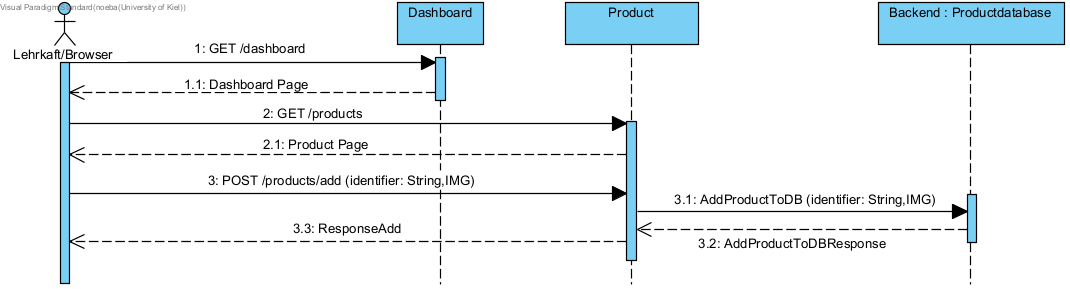
\includegraphics[width=\textwidth]{img/sequence-lehrkraft-add-product}
\label{fig: Lehrkraft Produkt hinzufügen Sequenzdiagramm}
Wir zeigen hier den Sequenzablauf für eine Lehrkraft, die ein Produkt ins System einführen möchte.\\
Nach dem Login und dem navigieren zur Produkt-Hinzufügungs-Oberfläche folgen über POST die Daten über das Produkt. Die Lehrkraft wird dann wieder auf die Ursprungsseite weitergeleitet, wo per popup eine Meldung gezeigt wird, die das Hinzufügen des Produktes bestätigt.


	\pagenumbering{gobble} % Nummerierung deaktivieren
\end{document}
